\pdfminorversion=4

\documentclass{beamer}
\usepackage[utf8]{inputenc}
%\usepackage[spanish]{babel}
\usepackage[english]{babel}

\usepackage{beamerthemeULoyola}
\usepackage{graphicx}
\usepackage{booktabs}

%% PRESENTATION CONFIGURATION PARAMETERS %%%%%%%%%%%%%%%%%%%%%%%%%%%%%%%%%%%%%%%
\titlebackgroundfile{images/template_title}
\framebackgroundfile{images/template_frame}
\definecolor{azulloyola}{HTML}{023E83}
\definecolor{azulloyolaclaro}{HTML}{9497B9}
\definecolor{gris}{HTML}{4C4C4C}
\definecolor{grisclaro}{HTML}{EBEBEB}
\definecolor{examplefrente}{HTML}{218E58}
\definecolor{examplefondo}{HTML}{C2D8CD}
\definecolor{alertfrente}{HTML}{FF0000}
\definecolor{alertfondo}{HTML}{E7BDBD}


\usefonttheme{structurebold}
\setbeamercolor{author in head/foot}{fg=white}
\setbeamercolor{title in head/foot}{fg=white}
\setbeamercolor{section in head/foot}{fg=azulloyola}
\setbeamercolor{normal text}{fg=gris}
\setbeamercolor{frametitle}{fg=azulloyola}
% \setbeamerfont{block title}{size={}}
\setbeamerfont{author}{size=\footnotesize}
\setbeamerfont{date}{size=\footnotesize}
\setbeamertemplate{itemize item}[circle]
\setbeamertemplate{itemize subitem}[triangle]
\setbeamertemplate{itemize subsubitem}[square]
\setbeamertemplate{itemize subsubsubitem}[ball]
\setbeamercolor{itemize item}{fg=azulloyola}
\setbeamercolor{itemize subitem}{fg=azulloyola}
\setbeamercolor{itemize subsubitem}{fg=azulloyola}
\setbeamercolor{itemize subsubsubitem}{fg=azulloyola}
\setbeamercolor{enumerate item}{fg=azulloyola}
\setbeamercolor{enumerate subitem}{fg=azulloyola}
\setbeamercolor{enumerate subsubitem}{fg=azulloyola}
\setbeamercolor{enumerate subsubsubitem}{fg=azulloyola}
% \setbeamercolor{alerted text}{fg=azulloyola}
% \setbeamerfont{alerted text}{series=\bfseries}

\setbeamertemplate{blocks}[shadow=true]
\setbeamercolor*{block title}{bg=azulloyolaclaro,fg=white}
\setbeamercolor*{block body}{bg=grisclaro,fg=gris}

\setbeamercolor*{block title example}{bg=examplefrente,fg=white}
\setbeamercolor*{block body example}{bg=examplefondo,fg=gris}

\setbeamercolor*{block title alerted}{bg=alertfrente,fg=white}
\setbeamercolor*{block body alerted}{bg=alertfondo,fg=gris}

\usecolortheme[named=azulloyola]{structure}


% This command makes that acrobat reader doesn't changes the colors of the slide
% when there are figures with transparencies.
\pdfpageattr {/Group << /S /Transparency /I true /CS /DeviceRGB>>}
%%%%%%%%%%%%%%%%%%%%%%%%%%%%%%%%%%%%%%%%%%%%%%%%%%%%%%%%%%%%%%%%%%%%%%%%%%%%%%%%

%      + Short title.               + Title which appears in the cover.
%      v                            v
\title[Diversity for ELM]{Diversity in Extreme Learning Machine ensembles}
%       + Short author names which appear in the slides.
%       v
\author[C. Perales-Gonz\'alez]
{   % Author names which appear in the cover page.
    Carlos Perales-Gonz\'alez\inst{1}
}
%          + Short affiliation which appears in the slides.
%          v
\institute[ULOYOLA]
{   % Affiliation information which appears in the cover page.
    \begin{tabular}{c}
    \inst{1}PhD student from Universidad Loyola Andaluc\'ia
    \end{tabular}
}
%     + Short acronym of the conference or date of the presentation.
%     v
\date[2018-4-4]
{   % Conference name which appears in the cover page.
%     Workshop with Peter Tino (2018).
Thesis directors: Francisco Fern\'andez-Navarro, David Becerra-Alonso, Mariano Carbonero-Ruz
}

\begin{document}
% Creates the cover page.
\frame{\titlepage}

\begin{frame}{Overview}
\tableofcontents
\end{frame}



\section{Introduction}
\subsection{What is machine learning?}

% 1
\frame{

\frametitle{Machine learning}

Machine learning: field of computer science that uses statistical techniques to give computer systems the ability to "learn" (i.e., progressively improve performance on a specific task) with data, without being explicitly programmed \cite{samuel1959some}.

\textbf{Machine learning is the study of pattern recognition}.

\begin{itemize}
  \item Unsupervised: inferring a hidden structure from unlabeled data. I.e.: Clustering, autoencoders neural networks, \ldots
  \item Supervised: learning a function that maps from features to target based on training data. I.e.: SVM, Ridge regression, decision tree, \ldots
    \begin{enumerate}
      \item Classification. Target is a category.
      \item Regression. Target is a real value.
    \end{enumerate}
\end{itemize}

}

% 2
\frame{

\frametitle{Supervised classification}

Algorithms minimize the error of classification. How?

\begin{itemize}
  \item Linear methods.
  \item Nonlinear methods.
    \begin{enumerate}
      \item Pure nonlinear methods. I.e.: Decision trees.
      \item Kernels. I.e.: RBF, polynomial.
    \end{enumerate}
\end{itemize}

%}
%
%
%% 2.2
%\frame{
%
%\frametitle{Analytic vs Heuristic}

How is the error function?

\begin{itemize}
  \item Heuristic. Constrain programming, huge and hard loss functions. I.e.: genetic or greedy algorithms.
  \item Analytic. Simpler algorithms, based on convex optimization. I.e.: SVM, ELM.
\end{itemize}

Convex optimization is fast.
But \textbf{strong assumption}: relation between features and target is convex.
\textbf{Solution}: ensembles.

}

%% 4
%\subsection{Kernel trick as feature space transformation}
%\frame{
%
%\frametitle{Kernel approach}
%
%What is kernel trick?
%
%Mathematical explanation. \textit{It exists an space where training data is linear separable, and that space is achievable not through a known transfer function but by inner product with the data of the space}.
%
%}


\section{Extreme Learning Machine / Ridge classification}
\subsection*{ELM}

% 1
\frame{

\frametitle{ELM I}

Extreme Learning Machine for classification, a.k.a. Ridge classification {\cite{hoerl1970ridge}, \cite{huang2006extreme}, \cite{huang2012extreme}}.

\begin{equation}
\label{eq:classification}
f(\boldsymbol{x}) = \boldsymbol{h}'\left(\boldsymbol{x}\right)\boldsymbol{\beta},
\end{equation}

where
\begin{itemize}
	\item $\boldsymbol{x} \in \mathbb{R}^{m}$ is the vector of attributes, $m$ is the dimension of the input space.
	\item $\boldsymbol{\beta} = (\boldsymbol{\beta}_{j}, j = 1,\ldots,J) \in \mathbb{R}^{d \times J}$ is ELM matrix.
	\item  $\boldsymbol{h} : \mathbb{R}^m \rightarrow \mathbb{R}^d$ is the mapping function and $d$ is the number of hidden nodes (the dimension of the transformed space).
\end{itemize}

% is the output matrix of coefficients, 
% the weights of the $j$-th output node, is the mapping function and $d$ is the number of hidden nodes (the dimension of the transformed space).
}

% 2
\frame{
	
\frametitle{ELM II}

\textbf{Learning problem}: Let us also denote $\boldsymbol{H}$ as $\boldsymbol{H}=\left({h}'\left(\boldsymbol{x}_{i}\right),\,i=1,\ldots,n\right)\in\mathbb{R}^{n \times d}$ as the transformation of the training set and $\boldsymbol{Y} \in \mathbb{R}^{n \times J}$ is the labels "1-of-J" encoded.

\begin{equation}
\label{eq:beta_jatrix}
\min_{\boldsymbol{\beta}\in \mathbb{R}^{d \times J} } \left({{\lVert \boldsymbol{\beta} \rVert}^2 +C \lVert \boldsymbol{H} \boldsymbol{\beta} - \boldsymbol{Y} \rVert}^2\right),
\end{equation}

where $C \in \mathbb{R}^{+}$ is a cross-validated hyper-parameter. % for regularization. Directly looking for minimizing errors.

\begin{equation}\label{eq:beta1}
\boldsymbol{\beta} = \left( \frac{\boldsymbol{I}}{C} +\boldsymbol{H}'\boldsymbol{H}\right)^{-1}\boldsymbol{H}'\boldsymbol{Y}
\end{equation}

}

% 3
\frame{
\frametitle{ELM III}

It uses:

\begin{itemize}
	\item Matrix programming.
	\item Use Tikhonov regularization.
\end{itemize}

Machine learning problems are not always solvable. To avoid inverse matrix problems, regularization term appears.

Different mapping functions $h$ haven been proposed

\begin{itemize}
\item Single Hidden Layer ELM, or Neural ELM.
\item Kernel ELM, or Kernel Ridge classification.
\end{itemize}

Proposed solution to avoid convex assumption: ensembles.
}


\section{Ensembles}
\subsection{State of art}

% 1
\frame{

\frametitle{Bagging and Boosting}
\textbf{Bagging} (bootstrap aggregating) is a learning method for generating several versions of a base learner by selecting some subsets from the training set and using these as new learning sets \cite{Bbeiman1996}. Random, different classifiers.

\textbf{Boosting} is a family of machine learning meta-algorithms which focus on combining base learners over several iterations and generate a weighted majority hypothesis \cite{Freund1997}.

}


\subsection{Diverse ensemble}
% \subsection*/{Diverse}

% 1
\frame{

\frametitle{Our proposal I}

Explicit diverse ensembles for classification. This was sent to the International Conference on Hybrid Artificial Intelligent Systems (HAIS) 2018 and accepted.

\begin{equation}
\label{eq:Diverse_ELM_min}
\min_{\boldsymbol{\beta}^{l}\in \mathbb{R}^{d \times J}}  \frac{1}{2}\left( {\lVert \boldsymbol{\beta}^{l} \rVert}^2 + C  {\lVert\boldsymbol{H}\boldsymbol{\beta}^{l}-\boldsymbol{Y}\rVert}^2 + \left(D+\frac n s\right)  \sum_{j=1}^J \sum_{k=1}^{l-1} \left\langle\boldsymbol{\beta}_{j}^{l} , \boldsymbol{u}_{j}^k\right\rangle^2 \right)
\end{equation}

where:
\begin{itemize}
\item $\boldsymbol{u}^k \in \mathbb{R}^{d \times J}$ is the column-by-column normalized $\boldsymbol{\beta}^k$ from the iteration $k$ of the ensemble.
\item $D >0$ is a hyper-parameter like $C$. 
\end{itemize}

}

\frame{
	
	\frametitle{Our proposal II}
	
Hence, $\boldsymbol{\beta}_{j}^{l}$ could be obtained analytically as:

\begin{equation}
\label{eq:beta_h_diverse_huge}
\boldsymbol{\beta}_{j}^{l}=\left(\frac{\boldsymbol{I}}{C}+\boldsymbol{H}'\boldsymbol{H}+\frac{1}{C}\left(D+\frac{n}{s}\right)\boldsymbol{M}_{j}^{l}\right)^{-1}\boldsymbol{H}'\boldsymbol{Y}_{j}\quad j=1,\ldots,J
\end{equation}
	
where $\boldsymbol{M}_{j}^l $ is defined as
\begin{equation}
\label{eq:M_j}
\boldsymbol{M}_{j}^l \equiv \sum_{k=1}^{l-1} \boldsymbol{u}_{j}^{k} \left(\boldsymbol{u}_{j}^{k}\right)'
\end{equation}
	
}

\frame{
	
\frametitle{Results I}

\begin{table}[H]
	\begin{scriptsize}
		\setlength{\tabcolsep}{7.8pt}
%		\caption{Test Diverse ELM and AdaBoost family, including the average over all the different splits}
		\begin{center}
			\begin{tabular}{c c c c c}
				\hline
				\hline
				&\multicolumn{4}{c}{Accuracy (Acc)}\\
				\cline{2-5}
				& DELM 					&	AELM		&	BRELM		&	NCELM  \\ 
				\hline 
				car				& $\textbf{0.929711}$ 	&	$0.834618$	&	$0.901805$	&	$\textit{0.905111}$ \\ 
				winequality-red	& $\textbf{0.853687}$	&	$\textit{0.840085}$	&	$0.839670$	& 	$0.837363$ \\ 
				ERA				& $\textbf{0.829479}$	&	$0.822201$	&	$0.828019$	&	$\textit{0.828428}$ \\ 
				LEV				& $\textbf{0.836345}$	&	$0.786404$	&	$0.792371$	&	$\textit{0.798220}$ \\ 
				SWD				& $\textbf{0.787940}$	&	$\textit{0.764487}$	&	$0.759893$	&	$0.760442$ \\ 
				newthyroid		& $\textbf{0.932035}$	&	$0.817172$	& 	$0.812035$	&	$\textit{0.819509}$ \\ 
				automobile		& $\textbf{0.867376}$	&	$0.834618$	&	$0.841636$	&	$\textit{0.846499}$ \\ 
				squash-stored	& $0.694286$	&	$\textbf{0.751429}$	&	$0.694063$	&	$\textit{0.711937}$ \\ 
				squash-unstored	& $\textit{0.814286}$	&	$\textbf{0.830952}$	&	$0.813810$	&	$0.812381$ \\ 
				pasture			& $\textbf{0.833333}$	&	$0.766667$	&	$0.811111$	&	$\textit{0.826667}$ \\ 
				\hline
				\hline \\
			\end{tabular}
		\end{center}
		\label{tab:results_acc}
	\end{scriptsize}
\end{table}

}


\frame{
	
	\frametitle{Results II}
	
	\begin{table}[H]
		\begin{scriptsize}
			\setlength{\tabcolsep}{7.8pt}
			%		\caption{Test Diverse ELM and AdaBoost family, including the average over all the different splits}
			\begin{center}
				\begin{tabular}{c c c c c}
\hline
\hline
&\multicolumn{4}{c}{Diversity (d)}\\
\cline{2-5}
& DELM					&	AELM		&	BRELM		&	NCELM  \\
\hline 
car				& $\textbf{0.999206}$ 	&	$0.180213$	&	$0.176621$	&	$\textit{0.181212}$ \\ 
winequality-red	& $\textbf{0.926890}$	&	$0.152451$	&	$0.124054$	& 	$\textit{0.185804}$ \\ 
ERA				& $\textbf{0.968917}$	&	$0.138991$	&	$0.143748$	&	$\textit{0.156551}$ \\ 
LEV				& $\textbf{0.992860}$	&	$0.098013$	&	$0.089886$	&	$\textit{0.133830}$ \\ 
SWD				& $\textbf{0.98095}3$	&	$0.130116$	&	$\textit{0.138222}$	&	$0.137884$ \\ 
newthyroid		& $\textbf{0.886023}$	&	$0.043061$	& 	$0.040141$	&	$\textit{0.057340}$ \\ 
automobile		& $\textbf{0.932272}$	&	$0.314529$	&	$0.311612$	&	$\textit{0.317588}$ \\ 
squash-stored	& $\textbf{0.668662}$	&	$0.216839$	&	$0.181023$	&	$\textit{0.217834}$ \\ 
squash-unstored	& $\textbf{0.568838}$	&	$0.130116$	&	$0.145780$	&	$\textit{0.155101}$ \\ 
pasture			& $0.081884$	&	$\textit{0.181297}$	&	$0.175300$	&	$\textbf{0.187400}$ \\ 
				\hline
				\hline \\
			\end{tabular}
		\end{center}
		\label{tab:results_div}
	\end{scriptsize}
\end{table}
}

% 2
\frame{

\frametitle{Motivation}



\begin{itemize}
\item Solve convex assumption, looking for local convexities.
\item Sensitivity analysis. It helps to establish a ranking of good solutions.
\item Diverse solutions are looked for in a explicit way.
\end{itemize}

}

% 3
\frame{
\frametitle{Work in progress}

Improving our proposal to HAIS 2018.

\begin{itemize}
\item More ensembles to compare against.
\item More data sets.
\item Minimizing runtime.
\item Sensitivity analysis.
\end{itemize}

}

\section{Future work}
% \subsection{Open source code}

\frame{
\frametitle{Framework in MATLAB (1)}

\begin{figure}[h!]
	
\includegraphics[width=100mm, height=60mm]{images/matlab_doc.png}
\end{figure}

}

\frame{
	\frametitle{Framework in MATLAB (2)}
	
	\begin{figure}[h!]
		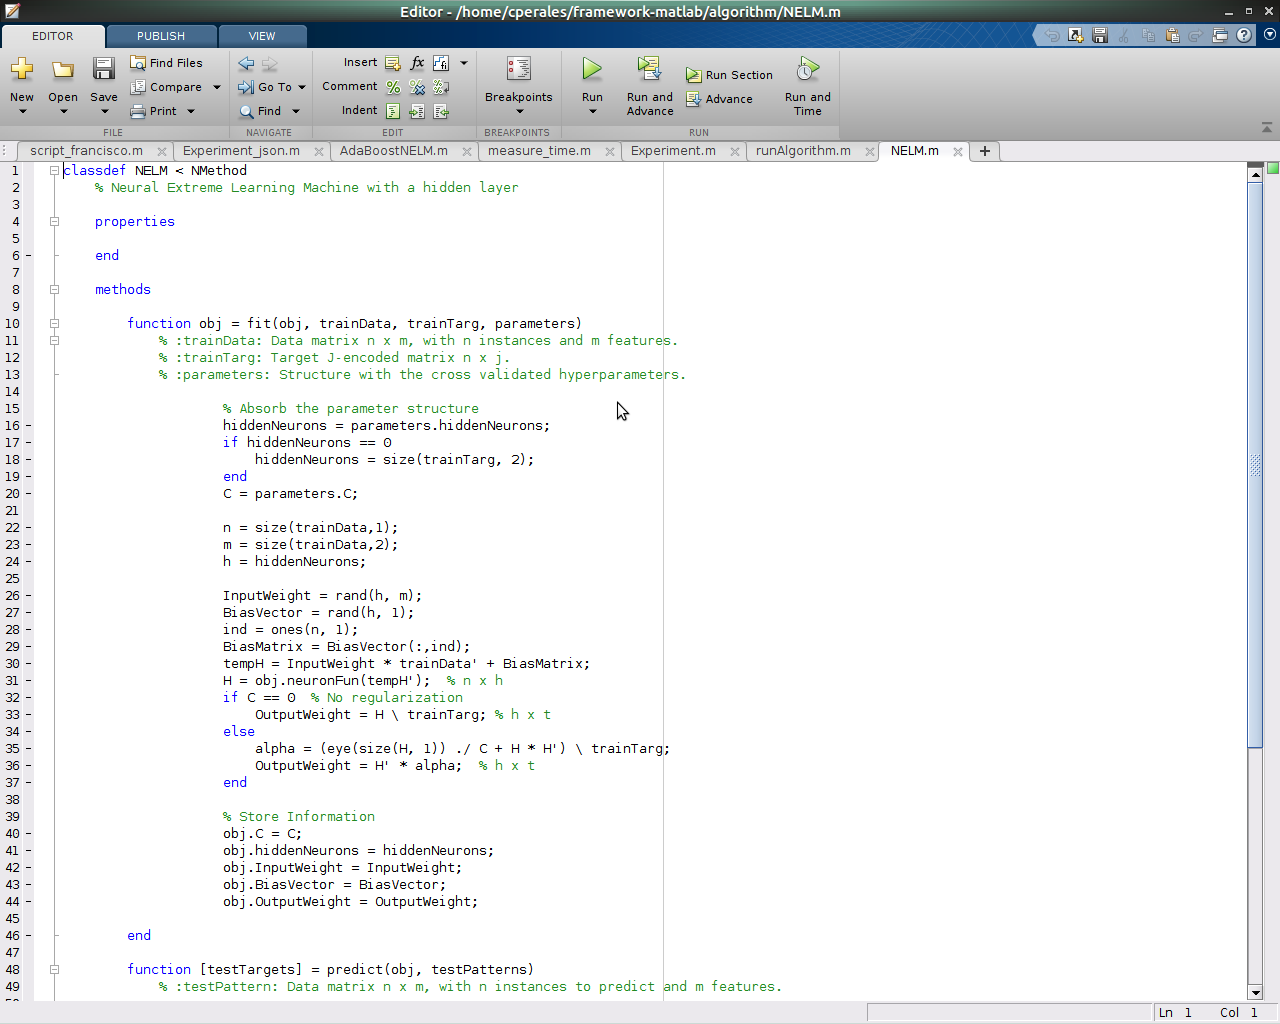
\includegraphics[width=100mm, height=60mm]{images/matlab_code.png}
	\end{figure}
	
}

\frame{
\frametitle{Framework in Python (1)}

\url{https://github.com/cperales/PyRidge}

	\begin{figure}[h!]
		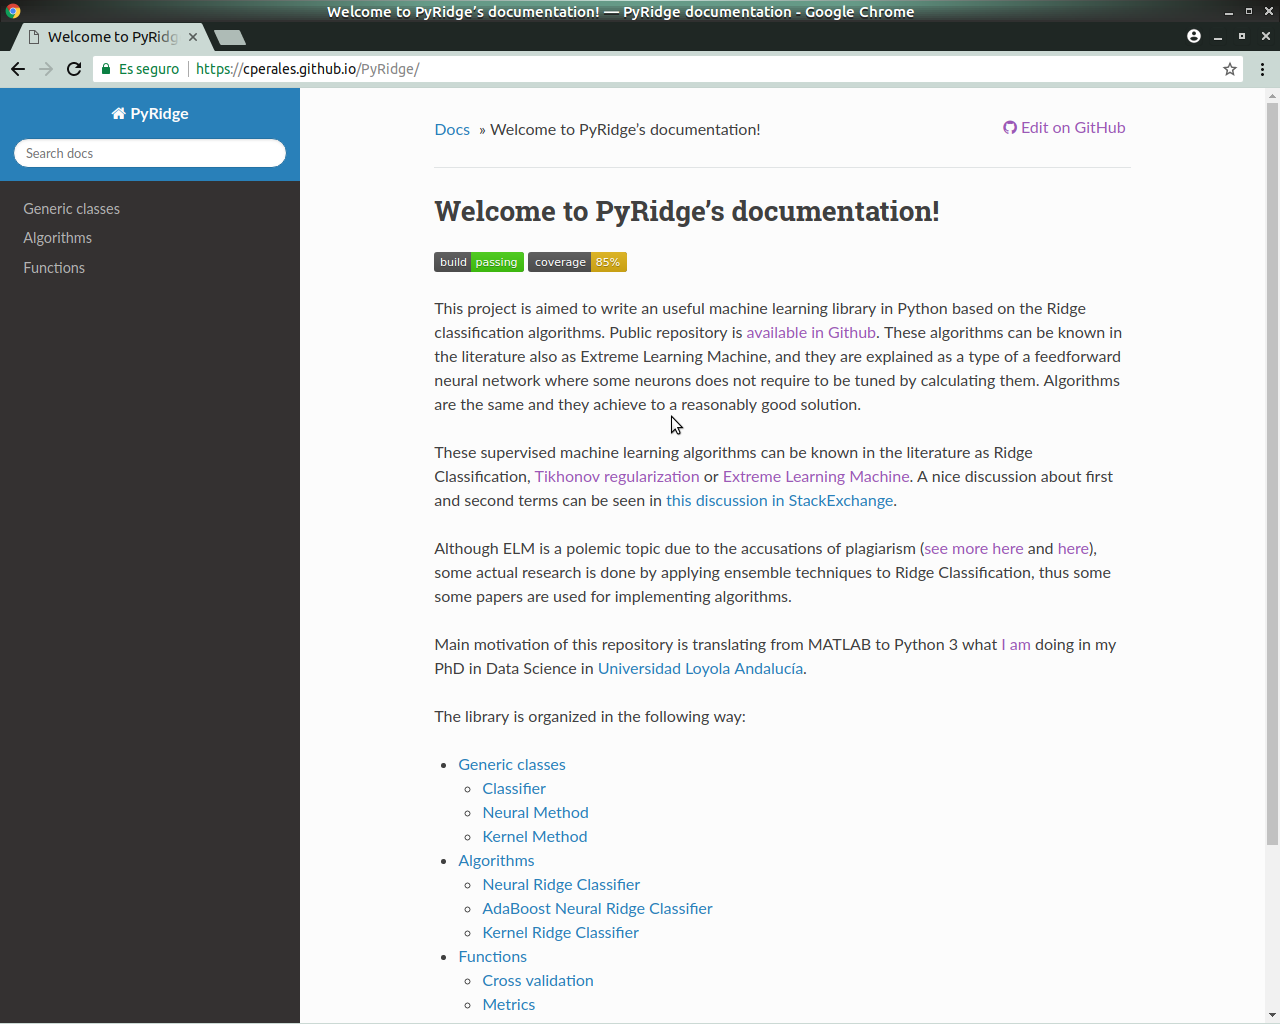
\includegraphics[width=100mm, height=60mm]{images/pyridge_doc.png}
	\end{figure}

}

\frame{
	\frametitle{Framework in Python (2)}
	
	\begin{figure}[h!]
		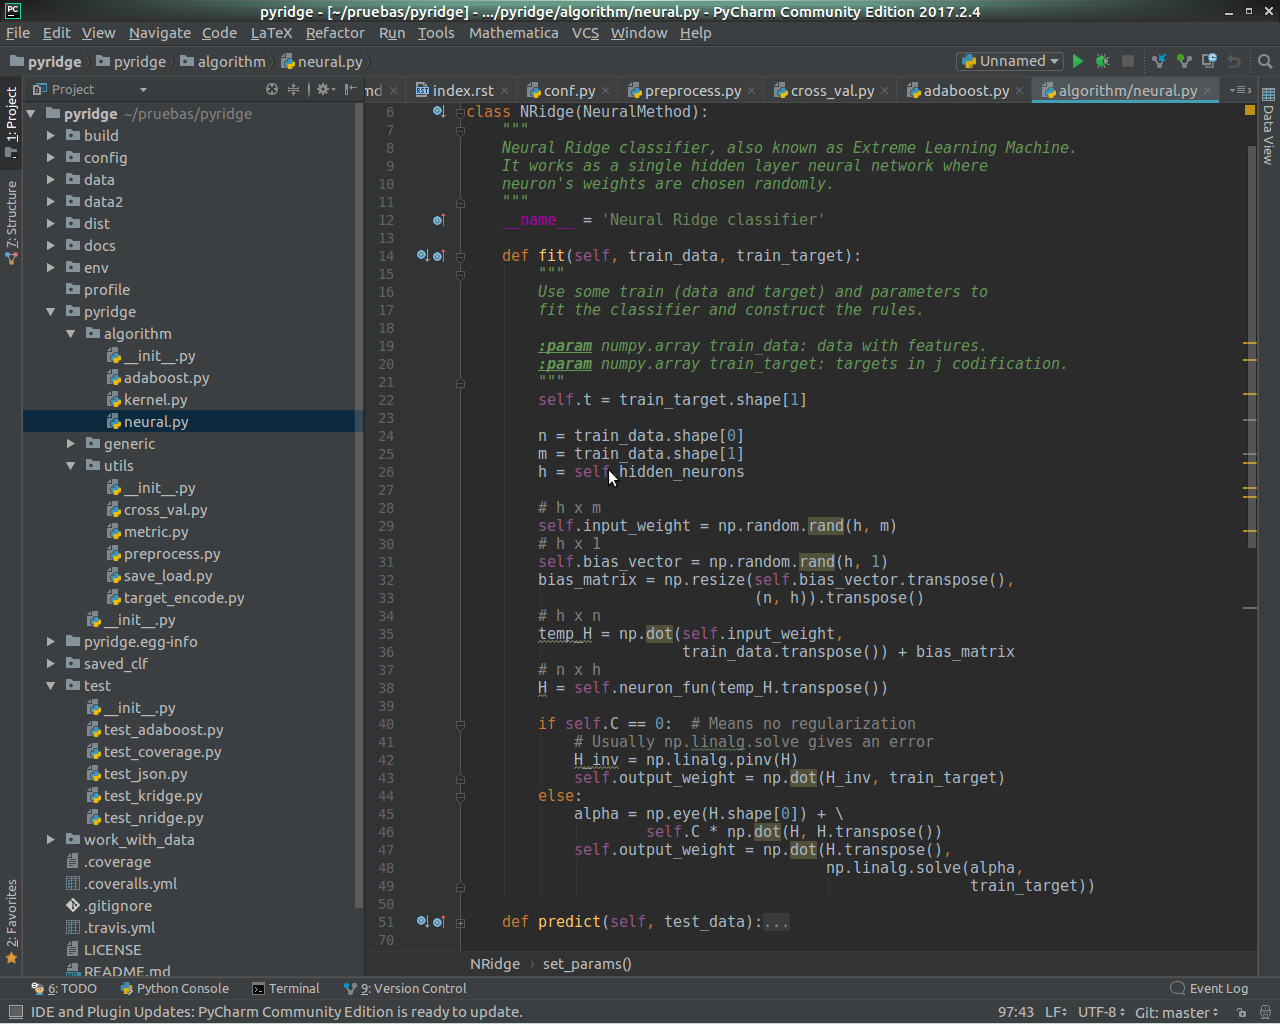
\includegraphics[width=100mm, height=60mm]{images/pyridge_code.png}
	\end{figure}
	
}

\frame{
\frametitle{scikit-learn / sklearn}

	\begin{figure}[h!]
		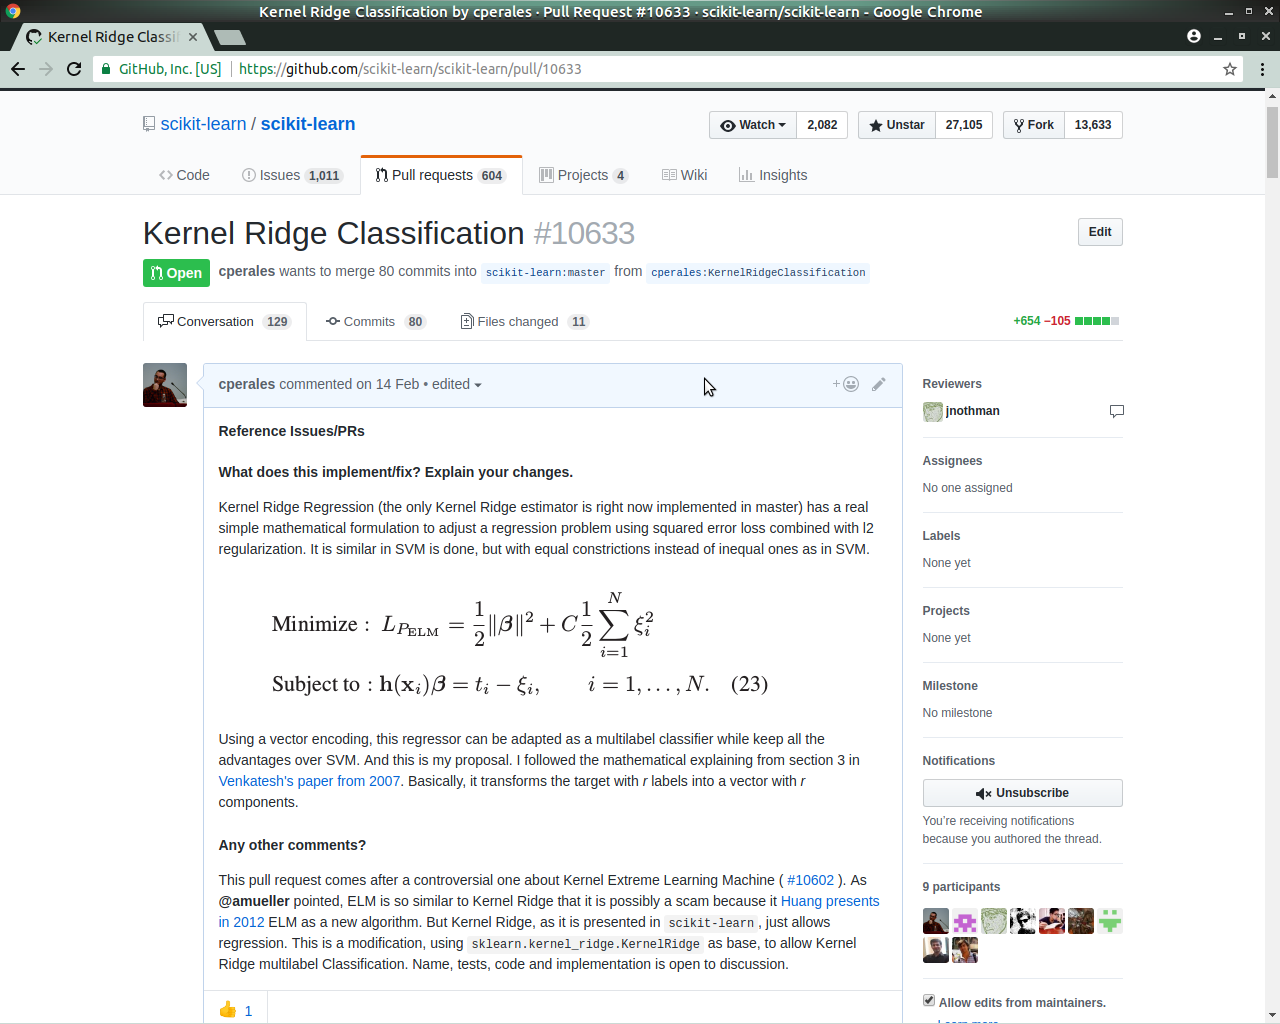
\includegraphics[width=100mm, height=60mm]{images/pull_request.png}
	\end{figure}

}

% \subsection{Collaboration}
% \frame{
% \frametitle{International collaboration}

% Guang-Bin Huang.

% Full Professor, Nanyang Technological University, Singapore.

% \begin{columns}
% 	\begin{column}{0.47\textwidth}
% 		\begin{itemize}
% 			\item Index h = 56.	
% 			\item Reviewing papers together.
% 			\item Possible JCR collaboration and international stay.
% 		\end{itemize}
% 	\end{column}
% 	\begin{column}{0.5\textwidth}
% 		\includegraphics{images/Huang_2.png}
% 	\end{column}
% \end{columns}
% }


\section*{Bibliography}
\begin{frame}[allowframebreaks]
	\frametitle{References}
    \bibliographystyle{ieeetr}
	\bibliography{workshop_bib.bib}
\end{frame}


\section*{END}
\frame{
	\frametitle{END}
\begin{center}
	\huge THANK YOU
\end{center}
}



\end{document}
